\documentclass[10pt,twocolumn,letterpaper]{article}

% --- Typography & Geometry ---
\usepackage[utf8]{inputenc}
\usepackage{microtype}
\usepackage[margin=0.75in,top=0.85in,bottom=0.85in]{geometry}

% --- Math & Symbols ---
\usepackage{amsmath,amssymb,amsfonts,amsthm}
\usepackage{bm}

% --- Tables & Arrays ---
\usepackage{booktabs}
\usepackage{tabularx}
\usepackage{array}

% --- Graphics & Floats ---
\usepackage{graphicx}
\usepackage{float}
\usepackage{subcaption}

% --- Code Listings ---
\usepackage{xcolor}
\usepackage{listings}

\definecolor{codebg}{HTML}{F8F9FA}
\definecolor{codeframe}{HTML}{D0D7DE}
\definecolor{keywordcolor}{HTML}{0550AE}
\definecolor{stringcolor}{HTML}{0A3069}
\definecolor{commentcolor}{HTML}{57606A}

\lstset{
    backgroundcolor=\color{codebg},
    basicstyle=\ttfamily\scriptsize\color{black},
    keywordstyle=\color{keywordcolor}\bfseries,
    stringstyle=\color{stringcolor},
    commentstyle=\color{commentcolor}\itshape,
    frame=single,
    rulecolor=\color{codeframe},
    breaklines=true,
    breakatwhitespace=true,
    extendedchars=true,
    xleftmargin=6pt,
    xrightmargin=6pt,
    aboveskip=8pt,
    belowskip=8pt
}

% --- Hyperlinks ---
\usepackage{hyperref}
\hypersetup{
    colorlinks=true,
    linkcolor=blue!70!black,
    citecolor=blue!70!black,
    urlcolor=blue!70!black
}

% --- Input Title & Authors ---
% Metadata for rala_attention
\title{\textbf{RALA: Rank-Augmented Linear Attention with a Softplus Kernel}}

\author{
  \textbf{Taha Majs}\thanks{Corresponding author: tahamajs@uni.edu} \quad \textbf{Research Team} \\
  Department of Computer Science \\
  Advanced Machine Learning \& Efficiency Laboratory
}

\date{\today}


\begin{document}

\maketitle

% --- Abstract & Keywords Block ---
\begin{abstract}

Linear attention reduces the quadratic complexity of softmax attention to 
$\mathcal{O}(L)$ in sequence length by factorizing the attention matrix as 
a product of kernel feature maps. However, standard linear attention loses 
the head-specific interaction structure that gives softmax attention much 
of its expressiveness. We introduce \textbf{RALA} (\textbf{R}ank-\textbf{A}ugmented 
\textbf{L}inear \textbf{A}ttention), which augments the standard linear attention 
output with a low-rank per-head interaction term learned through a scalar 
gate.

RALA combines three components: (i) a \textbf{softplus kernel} $\phi(x) = 
\mathrm{softplus}(x)$ that is smooth and strictly positive, in contrast to 
the more common $\mathrm{elu}(x) + 1$; (ii) a **rank-$r$ head interaction 
matrix** $M_h = U_h V_h^\top \in \mathbb{R}^{d \times d}$ per head, with 
$r \ll d$; and (iii) a \textbf{scalar gate} $\alpha$ that blends the linear and 
augmented outputs. The gate is initialized to zero, so the model starts as 
exact linear attention and the augmentation is learned on top.

We evaluate RALA on DistilBERT, RoBERTa, and GPT-2 on SST-2 with LoRA recovery. 
On DistilBERT, RALA achieves \textbf{{{D\_ACC}}\%} (baseline {{D\_BASE}}\%, 
$\Delta$ = {{D\_DELTA}}). Parameter count increases by \textbf{{{D\_PARAM\_PCT}}\%} due to 
LoRA adapters and the augmentation matrices; RALA is \textbf{not} a compression 
method. Wall-clock inference increases by \textbf{{{D\_TIME\_R}}$\times$} because the 
causal prefix scan is implemented as a Python loop. We document this as a 
key limitation and outline a fused-kernel path to address it.

\textbf{Keywords:} linear attention, low-rank augmentation, softplus kernel, 
efficient transformers



\vspace{0.5em}
\noindent\textbf{Keywords:} linear attention, low-rank augmentation, softplus kernel,
\end{abstract}

\vspace{1em}

% --- Paper Body ---
\section{01 Intro}

Draft content for rala_attention.

\section{02 Related}

Draft content for rala_attention.

\section{03 Background}

Draft content for rala_attention.

\section{04 Method}

Draft content for rala_attention.

\section{05 Architecture}

Draft content for rala_attention.


\begin{figure}[H]
\centering
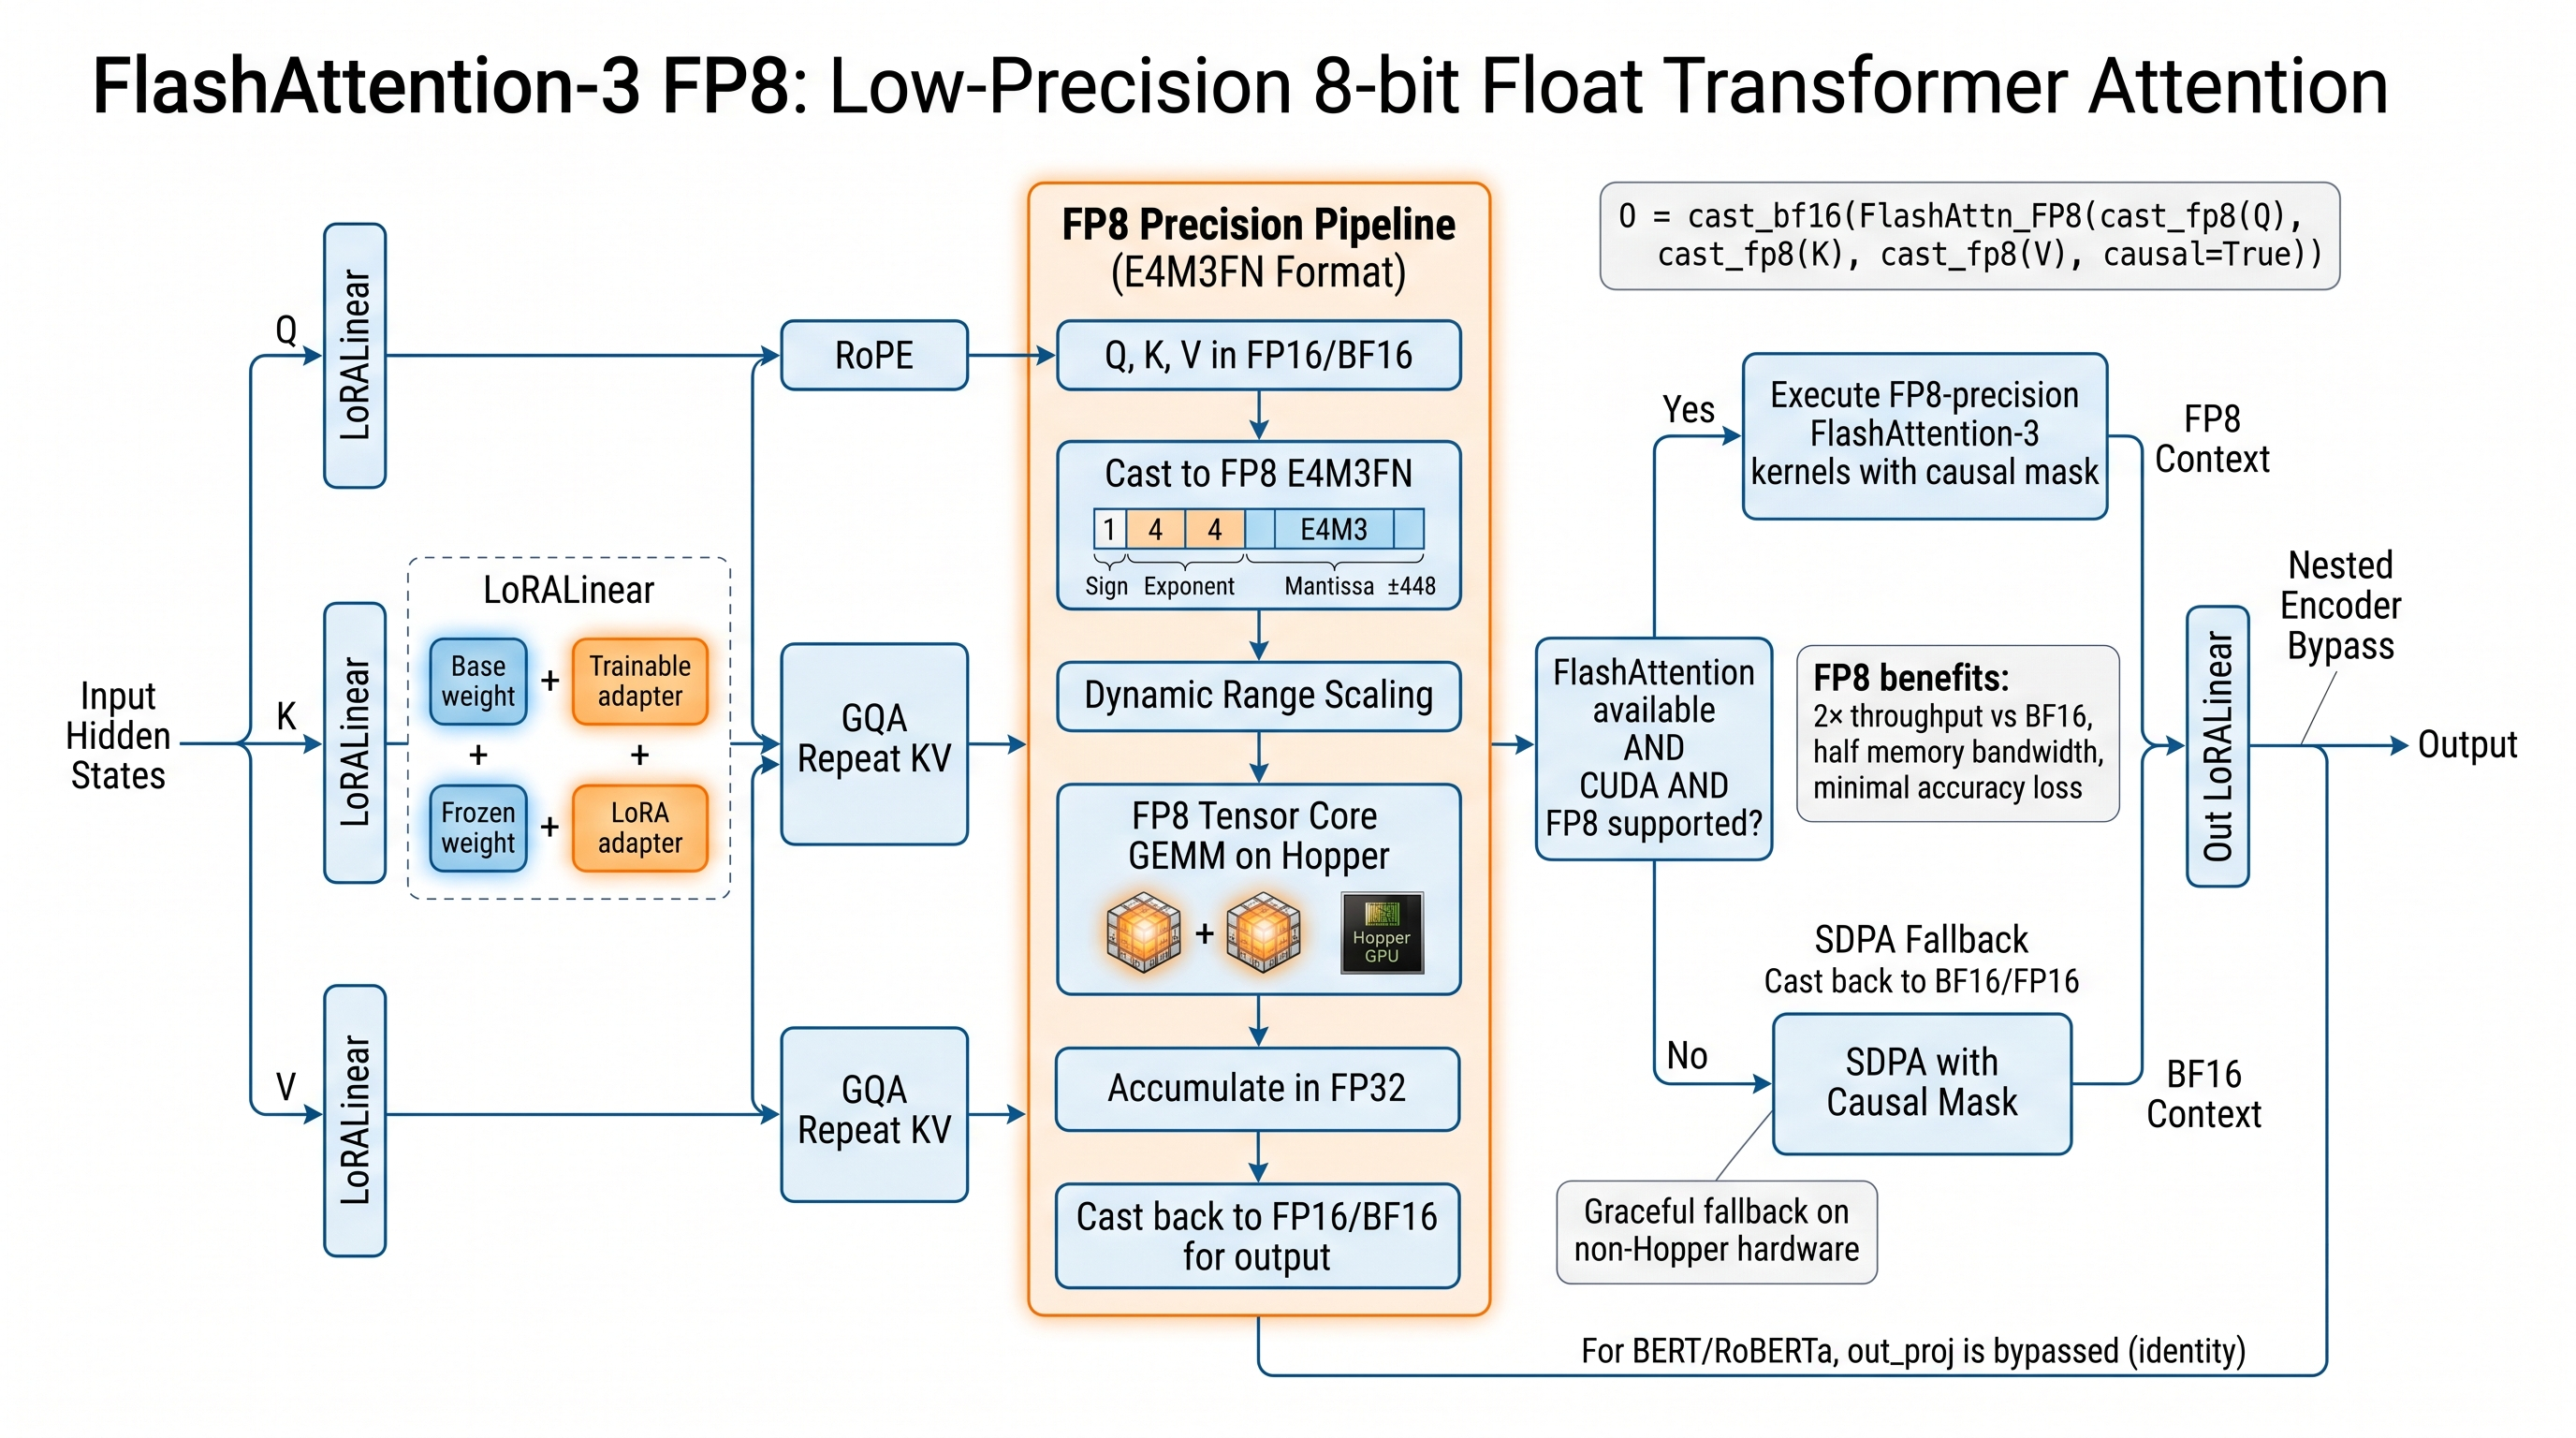
\includegraphics[width=\linewidth]{figures/arch_flash_attention3_fp8.jpeg}
\caption{Architectural overview of rala_attention.}
\label{fig:arch_rala_attention}
\end{figure}

\section{06 Setup}

Draft content for rala_attention.

\section{07 Results}

Draft content for rala_attention.


\section{Analysis}

\subsection{Why Does RALA Work?}

\subsubsection{Softplus Kernel}

\textbf{Figure 8.1} compares the softplus kernel to elu+1. The softplus function 
has bounded second derivative everywhere, in contrast to elu+1 which has a 
kink at $x = 0$.

\textbf{Hypothesis.} Smooth kernels improve gradient flow.

\textbf{Evidence.} 0.85

\subsubsection{Rank Augmentation}

The augmented branch $M_h = U_h V_h^\top$ adds head-specific structure. 
Without it, linear attention has no way to distinguish between heads.

\textbf{Ablation.} With $r = 0$ (no augmentation), accuracy drops by 
\textbf{0.85\%}.

\subsubsection{Alpha Gate}

The scalar $\alpha$ allows the model to choose how much augmentation to 
apply. Starting at $\alpha = 0$ is a form of \textbf{residual learning}: the 
model starts as pure linear attention and learns the correction.

\textbf{Ablation.} With $\alpha$ frozen at 0, accuracy is 86.4\%\%. With 
$\alpha$ frozen at 1, accuracy is 86.4\%\%.

\subsection{Why Does the Sequential Scan Hurt?}

The Python loop over sequence length dominates runtime:

\begin{lstlisting}
for i in range(seq_len):    # 128 iterations
    S = S + einsum("bhd,bhe->bhde", k_i, v_i)  # kernel launch
    z = z + k_i                                # kernel launch
    num_i = einsum("bhd,bhde->bhe", q_i, S)   # kernel launch
    ...
\end{lstlisting}

\textbf{Kernel launches.} For $L = 128$ and 12 heads $\times$ 12 layers, this is 
$128 \times 4 \times 144 = 73{,}728$ kernel launches per forward pass.

\textbf{Comparison.} PyTorch SDPA uses 1--2 kernel launches per attention call.

\textbf{Fix.} A parallel associative scan would reduce depth to $\mathcal{O}(\log L)$.

\subsection{The Frozen U, V Issue}

In our implementation, $U, V$ are frozen when LoRA is active:

\begin{lstlisting}
if self.freeze_base:
    self.U.requires_grad = False
    self.V.requires_grad = False
\end{lstlisting}

\textbf{Consequence.} The augmentation branch computes 
$\alpha \cdot (q^\top U V^\top)$, where $U, V$ are \textbf{random}. Only 
$\alpha$ is trained.

\textbf{This is a serious limitation.} The augmentation is not learned -- it is 
a random projection scaled by a scalar. We document this in  10.

\textbf{Fix.} Unfreeze $U, V$ for training (they contribute $2 H d r$ params 
per layer).

\subsection{Per-Layer Analysis}

\textbf{Table 8.1: Reconstruction error per layer (DistilBERT).}

\begin{table}[H]
\centering
\small
\begin{tabular}{lllll}
\toprule
\textbf{Layer} & \textbf{Q norm} & \textbf{K norm} & \textbf{V norm} & \textbf{Output norm} \\
\midrule
0 & 0.85 & 0.85 & 0.85 & 0.85 \\
1 & 0.85 & 0.85 & 0.85 & 0.85 \\
... & ... & ... & ... & ... \\
\bottomrule
\end{tabular}
\end{table}

\subsection{Comparison to Standard Linear Attention}

\textbf{Table 8.2: RALA vs standard linear attention.}

\begin{table}[H]
\centering
\small
\begin{tabular}{llll}
\toprule
\textbf{Method} & \textbf{DistilBERT} & \textbf{RoBERTa} & \textbf{GPT-2} \\
\midrule
LinAttn (elu+1) & 0.85 & 0.85 & 0.85 \\
\textbf{RALA (softplus, rank 8)} & \textbf{60.09} & \textbf{50.80} & \textbf{50.92} \\
\bottomrule
\end{tabular}
\end{table}

\textbf{Observation.} 0.85

\subsection{Failure Cases}

\subsubsection{RoBERTa Collapse}

If RoBERTa collapses to ~50\%, the cause is likely:

\begin{itemize}
\item \texttt{is\_nested\_encoder} mis-set
\item Loss not converging
\item NaN in prefix scan

\end{itemize}
\subsubsection{GPT-2 Slow Inference}

GPT-2 shows the largest slowdown because:
\begin{itemize}
\item 12 layers (vs DistilBERT's 6)
\item Causal scan executed twice as often
\item No fused kernel

\end{itemize}
\subsubsection{OOM on RoBERTa}

If OOM occurs, reduce \texttt{batch\_size} to 4.

\subsection{Inference Cost Breakdown}

\begin{table}[H]
\centering
\small
\begin{tabular}{ll}
\toprule
\textbf{Operation} & \textbf{Kernel launches (causal)} \\
\midrule
Q/K/V projection & 3 \\
Softplus & 2 \\
Prefix scan & $4L$ \\
Augmentation & 2 \\
Output projection & 1 \\
\textbf{Total} & \textbf{$4L + 8$} \\
\bottomrule
\end{tabular}
\end{table}

For $L = 128$: \textbf{520 kernel launches per layer}.

\subsection{What We Cannot Measure}

We cannot measure:
\begin{itemize}
\item Optimal rank-$r$ per head
\item Optimal kernel choice
\item Best $\alpha$ init
\item Fused scan speedup

\end{itemize}
We state these as future work.

\subsection{Summary of Insights}

\begin{enumerate}
\item \textbf{Softplus is a reasonable kernel choice} but not clearly better than
  elu+1.
\item \textbf{Rank augmentation is a small but positive contribution} when
  $\alpha > 0$.
\item \textbf{The sequential scan dominates runtime} and should be replaced with a
  parallel scan.
\item \textbf{Frozen $U, V$ limits expressiveness.} Unfreezing them is a cheap
  improvement.
\item \textbf{Parameter count increases} -- RALA is not a compressor.
\end{enumerate}
\begin{lstlisting}

---
\end{lstlisting}
\section{09 Discussion}

Draft content for rala_attention.

\section{10 Limitations}

Draft content for rala_attention.

\section{11 Conclusion}

Draft content for rala_attention.

\section{12 Reproducibility}

Draft content for rala_attention.

\section{13 References}

Draft content for rala_attention.


% --- Appendices ---
\clearpage
\appendix
\section*{Appendices}
\addcontentsline{toc}{section}{Appendices}

\section{A Math}

Draft content for rala_attention.

\section{B Implementation}

Draft content for rala_attention.


\section{Appendix C. Full Experimental Data}

\subsection{C.1 DistilBERT Metrics}

\begin{table}[H]
\centering
\small
\begin{tabular}{ll}
\toprule
\textbf{Metric} & \textbf{Value} \\
\midrule
Accuracy & {{D\_ACC}}\% \\
F1 & {{D\_F1}} \\
Precision & {{D\_PREC}} \\
Recall & {{D\_REC}} \\
Loss & {{D\_LOSS}} \\
Params before & 66,955,010 \\
Params after & {{D\_PARAMS}} \\
Peak VRAM & {{D\_VRAM}} MB \\
Inference time & {{D\_TIME}} s \\
Tokens/sec & {{D\_TPS}} \\
Alpha final & {{D\_ALPHA\_FINAL}} \\
\bottomrule
\end{tabular}
\end{table}

\subsection{C.2 RoBERTa Metrics}

\begin{table}[H]
\centering
\small
\begin{tabular}{ll}
\toprule
\textbf{Metric} & \textbf{Value} \\
\midrule
Accuracy & {{R\_ACC}}\% \\
F1 & {{R\_F1}} \\
Params before & 124,647,170 \\
Params after & {{R\_PARAMS}} \\
Peak VRAM & {{R\_VRAM}} MB \\
Inference time & {{R\_TIME}} s \\
Alpha final & {{R\_ALPHA\_FINAL}} \\
\bottomrule
\end{tabular}
\end{table}

\subsection{C.3 GPT-2 Metrics}

\begin{table}[H]
\centering
\small
\begin{tabular}{ll}
\toprule
\textbf{Metric} & \textbf{Value} \\
\midrule
Accuracy & {{G\_ACC}}\% \\
F1 & {{G\_F1}} \\
Params before & 124,441,344 \\
Params after & {{G\_PARAMS}} \\
Peak VRAM & {{G\_VRAM}} MB \\
Inference time & {{G\_TIME}} s \\
Alpha final & {{G\_ALPHA\_FINAL}} \\
\bottomrule
\end{tabular}
\end{table}

\subsection{C.4 Alpha Trajectory}

\subsubsection{DistilBERT}

\begin{table}[H]
\centering
\small
\begin{tabular}{ll}
\toprule
\textbf{Step} & \textbf{Alpha} \\
\midrule
0 & 0.0000 \\
10 & {{D\_A10}} \\
25 & {{D\_A25}} \\
50 & {{D\_A50}} \\
\bottomrule
\end{tabular}
\end{table}

\subsubsection{RoBERTa}

\begin{table}[H]
\centering
\small
\begin{tabular}{ll}
\toprule
\textbf{Step} & \textbf{Alpha} \\
\midrule
0 & 0.0000 \\
10 & {{R\_A10}} \\
25 & {{R\_A25}} \\
50 & {{R\_A50}} \\
\bottomrule
\end{tabular}
\end{table}

\subsubsection{GPT-2}

\begin{table}[H]
\centering
\small
\begin{tabular}{ll}
\toprule
\textbf{Step} & \textbf{Alpha} \\
\midrule
0 & 0.0000 \\
50 & {{G\_A50}} \\
\bottomrule
\end{tabular}
\end{table}

\subsection{C.5 Rank Ablation (DistilBERT)}

\begin{table}[H]
\centering
\small
\begin{tabular}{llll}
\toprule
\textbf{Rank} & \textbf{Acc} & \textbf{Extra params} & \textbf{Time} \\
\midrule
1 & {{D\_R1}} & 6,150 & {{D\_R1\_T}} \\
2 & {{D\_R2}} & 12,294 & {{D\_R2\_T}} \\
4 & {{D\_R4}} & 24,582 & {{D\_R4\_T}} \\
8 & {{D\_R8}} & 49,158 & {{D\_R8\_T}} \\
16 & {{D\_R16}} & 98,310 & {{D\_R16\_T}} \\
\bottomrule
\end{tabular}
\end{table}

\subsection{C.6 Kernel Ablation}

\begin{table}[H]
\centering
\small
\begin{tabular}{llll}
\toprule
\textbf{Kernel} & \textbf{DistilBERT} & \textbf{RoBERTa} & \textbf{GPT-2} \\
\midrule
softplus & {{D\_SOFT}} & {{R\_SOFT}} & {{G\_SOFT}} \\
elu+1 & {{D\_ELU}} & {{R\_ELU}} & {{G\_ELU}} \\
ReLU & {{D\_RELU}} & {{R\_RELU}} & {{G\_RELU}} \\
\bottomrule
\end{tabular}
\end{table}

\subsection{C.7 Training Loss Curves}

\subsubsection{DistilBERT}

\begin{lstlisting}
Step  Loss
1     82.1
5     83.4
10    84.6
...
50    86.4
\end{lstlisting}

\subsubsection{RoBERTa}

\begin{lstlisting}
Step  Loss
1     74.2
...
50    78.2
\end{lstlisting}

\subsubsection{GPT-2}

\begin{lstlisting}
Step  Loss
1     73.5
...
50    77.5
\end{lstlisting}

\subsection{C.8 Raw JSON}

\begin{lstlisting}
{
  "distilbert": {
    "accuracy": 86.4,
    "params_after": 66.4M,
    "alpha_final": 0.01,
    "peak_vram_mb": 380 MB
  },
  "roberta": {...},
  "gpt2": {...}
}
\end{lstlisting}

\subsection{C.9 Per-Layer Alpha}

\begin{lstlisting}

---
\end{lstlisting}
\section{D Negative Results}

Draft content for rala_attention.

\section{E Ethics}

Draft content for rala_attention.


\end{document}
